
\chapter{Xilinx 7系列FPGA和IP核的使用}
\begin{introduction}
  \item \textit{Clocking Wizard IP Core}的使用
  \item \textit{DDS Compiler IP Core}的使用
  \item \textit{Integrated Logic Analyzer(ILA) IP Core}的使用
  \item 调用\textit{IP}核输出余弦信号到实验平台
\end{introduction}
\section{实验背景与目的}
随着 FPGA(Field Programmable Gate Array)技术的快速发展,基于 FPGA 的数字信号处理、嵌入式系统和高性能计算得到了广泛应用。Xilinx 7 系列 FPGA 作为当前主流的可编程逻辑器件之一,提供了丰富的硬件资源和灵活的开发环境。Vivado 设计套件(Vivado Design Suite)作为 Xilinx 提供的综合开发工具,支持 FPGA 设计、仿真、调试以及 IP 核的集成,极大地提高了开发效率。

在 FPGA 设计过程中,IP(Intellectual Property)核作为一种预先设计好的模块,提供了高效、可靠的硬件功能封装。通过调用 Xilinx 提供的 IP 核,开发者可以快速实现复杂的功能,例如时钟管理(Clocking Wizard)、数字信号处理(DDS Compiler)、片上调试(Integrated Logic Analyzer, ILA)等,从而减少低级电路设计的复杂性,提高开发效率。

本实验通过 Xilinx 7 系列 FPGA 及 Vivado 设计环境,介绍如何使用和配置常见的 IP 核,并结合具体应用场景,实现特定功能,如时钟信号的生成、余弦波信号的合成以及片上逻辑分析等。

\section{实验原理}
\subsection{IP 核}
\begin{definition}[IP核]
  Xilinx 提供了一系列 IP 核(Intellectual Property Cores),这些是可复用的硬件模块,用于加速 FPGA 设计开发。IP 核可以是预先优化的逻辑电路,如 DSP 处理单元、存储接口、AXI 总线接口等。使用 IP 核可以减少设计时间,提高 FPGA 资源利用率,并优化性能。
\end{definition}


Xilinx IP 核主要包括数学计算(DDS Compiler、CORDIC)、信号处理(FIR Compiler、FFT)、存储管理(BRAM Controller、FIFO Generator)、通信接口(AXI Interconnect、UART、SPI)、DSP 加速(DSP Slice、HLS 生成的 IP)、时钟管理(Clocking Wizard、PLL)等类别。

在 Vivado 中,用户可以通过 \texttt{IP Catalog} 选择合适的 IP 核,配置输入/输出接口、数据位宽和时钟频率,并生成 RTL 代码。然后,可以在 Verilog 代码中实例化该 IP 核,例如:
\begin{lstlisting}[language=verilog]
dds_compiler_0 my_dds (
    .aclk(clk), 
    .s_axis_config_tvalid(1'b1),  
    .s_axis_config_tdata(16'H51E), 
    .m_axis_data_tvalid(),   
    .m_axis_data_tdata(sin_out) 
);
\end{lstlisting}

此外,用户可以使用 Xilinx Vitis HLS 通过 C++ 代码生成 IP 核,例如:
\begin{lstlisting}[language=C++]
void my_ip(ap_fixed<16,8> in, ap_fixed<16,8> &out) {
    out = in * 1.5;
}
\end{lstlisting}
然后在 Vivado 中综合并调用。

由于 Icarus Verilog(iverilog)不支持直接仿真 Xilinx IP 核,推荐使用 Vivado 自带的 \texttt{xsim} 进行仿真,或者手写 Verilog 模型替代 IP 核。

综上所述,Xilinx IP 核能够显著加速 FPGA 设计,减少手写代码量,提高设计效率。用户可以根据具体需求选择合适的 IP 核,并结合 HLS 技术优化 FPGA 设计流程。
\subsection{调用 IP 核的一般方法}

在 FPGA 设计中,IP 核的调用通常分为以下几个步骤:IP 选择、参数配置、实例化、综合及仿真。Xilinx 提供的 IP 核可以通过 Vivado 进行管理,用户可以根据需要调用适当的 IP 核,提高开发效率。

首先,在 Vivado 中打开 \texttt{IP Catalog},搜索所需的 IP 核,例如 \texttt{DDS Compiler} 生成余弦波,\texttt{FIFO Generator} 用于数据缓存,\texttt{AXI Interconnect} 用于总线连接等。用户可以双击 IP 核进入配置界面,调整数据位宽、时钟频率、接口类型等参数。

配置完成后,点击 \texttt{Generate} 生成相应的 RTL 代码和示例文件。生成的文件通常包括 HDL 代码、仿真模型和 IP 的 \texttt{xci} 配置文件。在 Verilog 或 VHDL 代码中,用户需要实例化该 IP 核,例如对一个FIFO模块的例化:
\begin{lstlisting}[language=verilog]
fifo_generator_0 my_fifo (
    .clk(clk),
    .srst(reset),
    .din(data_in),
    .wr_en(write_enable),
    .rd_en(read_enable),
    .dout(data_out),
    .full(full),
    .empty(empty)
);
\end{lstlisting}

综合(Synthesis)和实现(Implementation)完成后,可以使用 \texttt{xsim} 进行仿真,或者直接下载到 FPGA 进行调试。如果需要与上层软件交互,可以通过 \texttt{AXI} 接口连接处理器(如 MicroBlaze 或 ARM 核),并在 Vitis 软件环境中编写驱动代码。例如,使用 Xilinx 提供的 API 访问 FIFO:
\begin{lstlisting}[language=C++]
Xil_Out32(FIFO_BASEADDR, data);
data = Xil_In32(FIFO_BASEADDR);
\end{lstlisting}


\section{实验使用软件/平台}
\begin{itemize}
  \item Xilinx Vivado 2023.2;
  \item eNodeX 30B软件无线电创新平台;
  \item 示波器。
\end{itemize}
\section{实验内容}
\subsection{Clocking Wizard IP Core配置50MHz时钟信号}
这个IP核用来生成50MHz时钟频率的同步时钟信号。在IP Catalog中搜索\textit{Clocking Wizard} IP核。修改配置如图~\ref{fig:exp3:clk-1}~所示。在Output Clocks栏里去除复位信号,保留使能信号Lock,指定一个频率为50MHz的时钟输出\texttt{clk\_out\_50m}。生成模块后,复制IP核提供的例化模块信息到待测模块中即可。

\begin{figure}[htbp]
  \centering
  \subfloat[模块时钟输入]{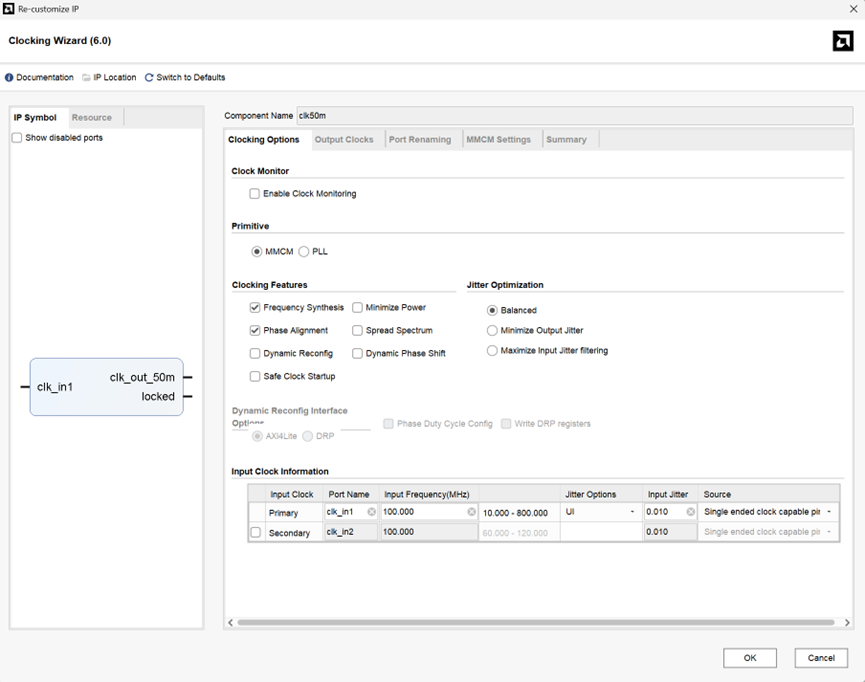
\includegraphics[width=0.45\textwidth]{figure/exp3/clk-1.png}}
  \hfill
  \subfloat[模块接口配置]{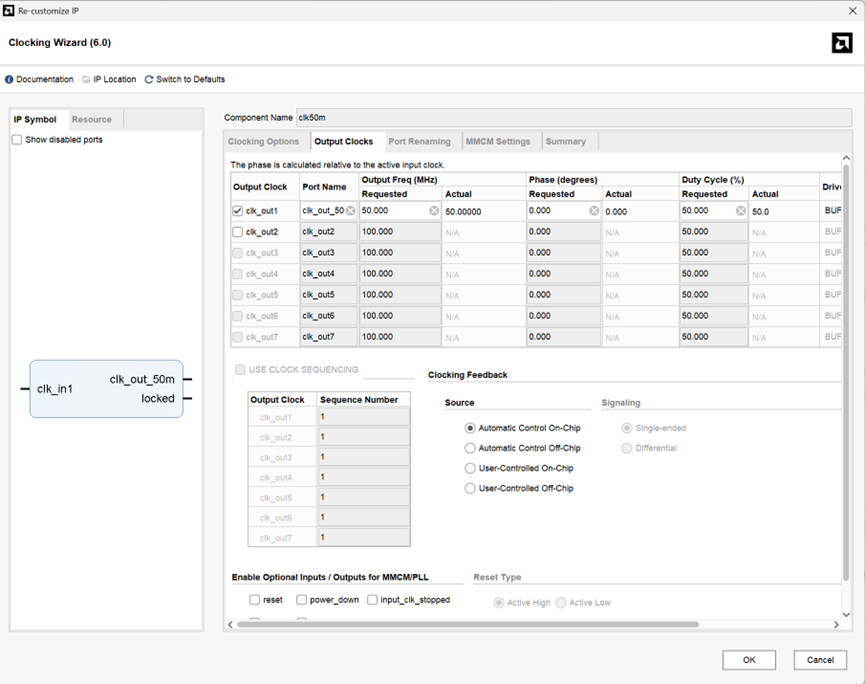
\includegraphics[width=0.45\textwidth]{figure/exp3/clk-2.png}}
  \caption{Clocking Wizard 配置信息}
  \label{fig:exp3:clk-1}
\end{figure}



\subsection{DDS Compiler IP Core配置1MHz和2MHz的余弦波}
在IP Catalog中搜索\textit{DDS Compiler} IP核。Vivado会自动弹出配置窗口。修改配置如图~\ref{fig:exp3:dds-1}~所示。由于同步时钟为50MHz,故DDS的时钟频率也需要和同步时钟频率相同;适当提高其无杂散动态范围 (SFDR, Spurious Frequency Dynamic Range)用来生成有用分量占比更大的余弦信号。配置结束后,将Output Frequency分别设置为1MHz和2MHz,例化两个模块。\footnote{实际的输出频率会略低于设定频率,这是由于DDS使用14-bit量化方案存储,会产生一定的量化误差。}
\begin{figure}[htbp]
  \centering
  \subfloat[模块配置]{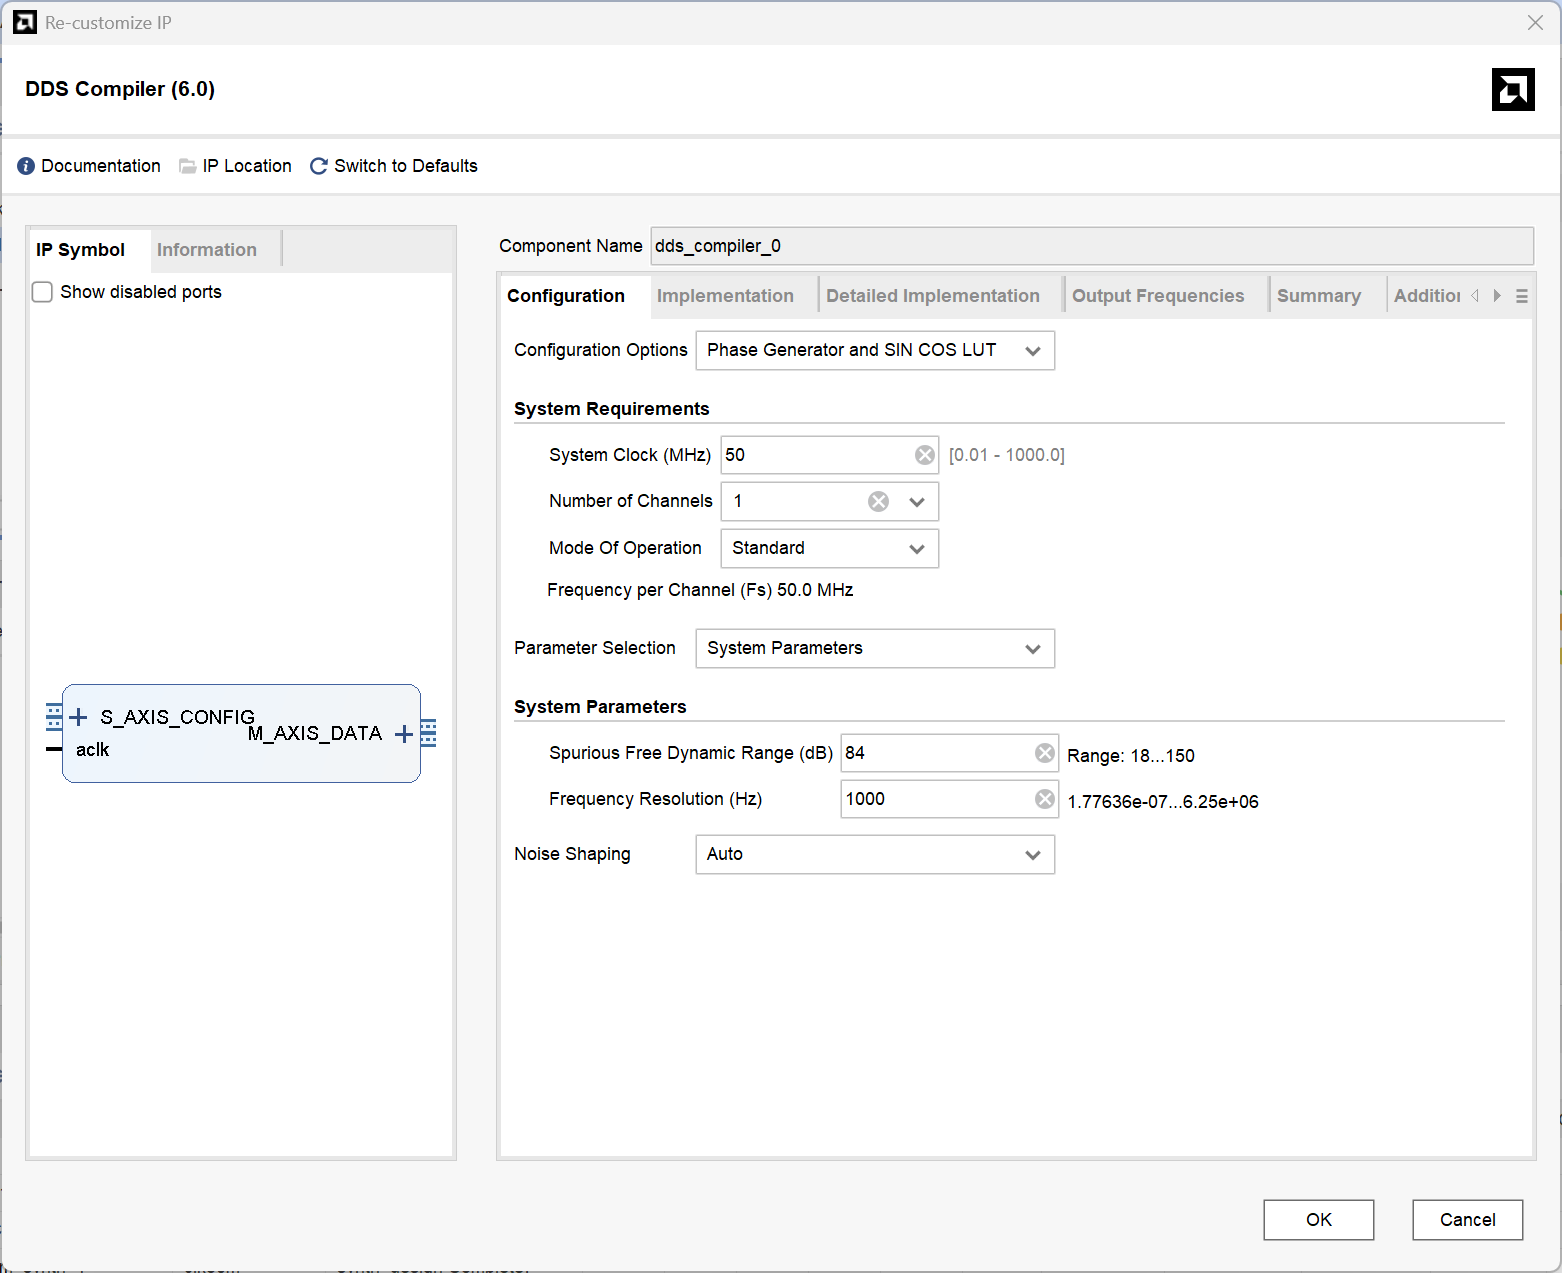
\includegraphics[width=0.45\linewidth]{figure/exp3/dds-1.png}}
  \hfill
  \subfloat[模块构建信息]{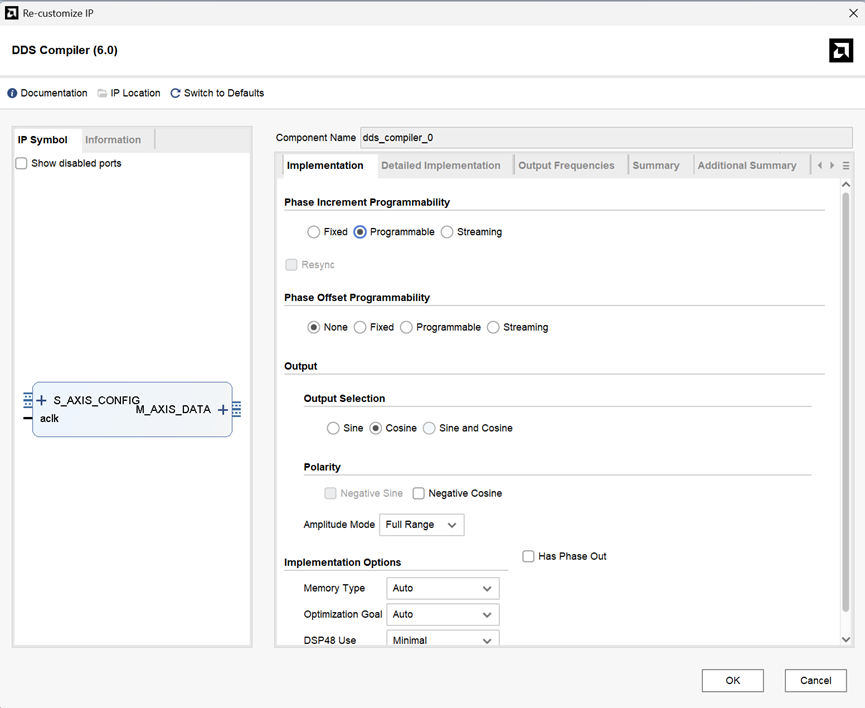
\includegraphics[width=0.45\linewidth]{figure/exp3/dds-2.png}}
  \caption{DDS Compiler配置信息}
  \label{fig:exp3:dds-1}
\end{figure}

\subsection{Integrated Logic Analyzer(ILA) IP Core配置}

Integrated Logic Analyzer(ILA)是 Xilinx 提供的一种片上调试工具,用于实时监测 FPGA 内部信号。ILA IP 核可以与 Vivado 逻辑分析仪(Logic Analyzer)协同工作,在不影响电路运行的情况下捕获关键信号,方便用户进行调试。

配置时,首先在 Vivado 的 \texttt{IP Catalog} 中搜索 \texttt{ILA},双击打开 IP 配置界面。在配置页面,用户设置以下参数:
\begin{itemize}
    \item \textbf{Probe 端口数量}:指定需要监测的信号数量,这里指定DAC之前的数字信号端口,\texttt{probe0}和\texttt{probe1}用来检测两种频率的余弦波。
    \item \textbf{每个 Probe 端口的数据宽度}:设置每个监测信号的位宽,通常与目标信号匹配。由于DAC的输出位宽为14-bit,此处位宽为14。
    \item \textbf{采样时钟}:ILA 需要连接 FPGA 内部的时钟信号,选择50MHz的系统时钟。
\end{itemize}

配置结束后,设置页面的参数如图~\ref{fig:exp3:ILA}~所示。
\begin{figure}[htbp]
  \centering
  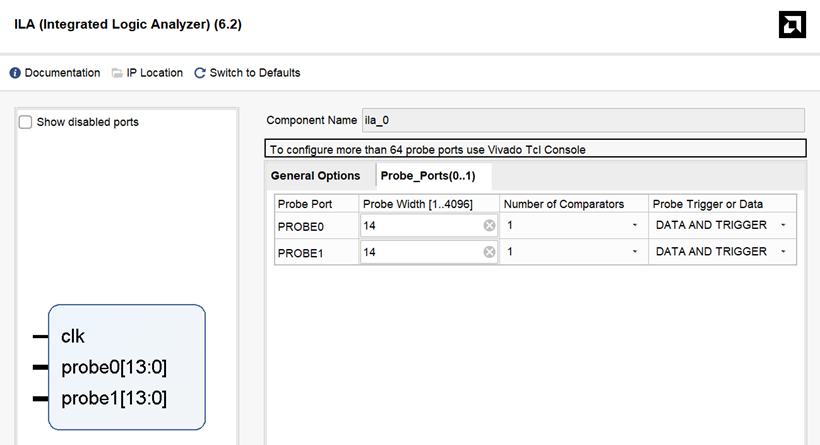
\includegraphics[width=0.75\textwidth]{figure/exp3/ila.png}
  \caption{ILA的IP核设置}
  \label{fig:exp3:ILA}
\end{figure}

在综合(Synthesis)和实现(Implementation)之后,用户需要生成比特流(Bitstream)。下载至 FPGA 后,打开 Vivado 的硬件管理器(Hardware Manager),连接开发板,加载比特流文件,就可以在右侧端口启动 ILA 仿真。


\subsection{利用IP核生成不同频率的余弦信号}
使用上述三个IP核的配置,编写Verilog代码:
\begin{lstlisting}[language=verilog]
`timescale 1ns / 1ps
module top_mod
(
	// DAC  PINS
  input PL_CLK_100MHz, 
  output signed [13:0] LS_DAC2_DB,   
	output LS_DAC2_CLK,              
	output LS_DAC2_WRT,         
	output signed [13:0] LS_DAC1_DB, 
  output LS_DAC1_CLK, 
	output LS_DAC1_WRT,
	output LS_DAC_MODE
);

	wire  clk_50M;                              // Storage of Clock
	wire clk_locked;                            // lock signal for clk
	wire signed [13:0] sin1M_data, sin2M_data;  // Storage of sine waves
	
	clk50m CLK_50M
    (
      // Clock out ports
      .clk_out_50m(clk_50M),     // output clk_out_50m
      // Status and control signals
      .locked(clk_locked),       // output locked
     // Clock in ports
      .clk_in1(PL_CLK_100MHz)      // input clk_in1
    );
    
  dds_compiler_0 DDS_1M_GENERATOR 
    (
      .aclk(clk_50M),                                  // input wire aclk
      .s_axis_config_tvalid(1'b1),  // input wire s_axis_config_tvalid
      .s_axis_config_tdata(16'H51E),    // input wire [15 : 0] s_axis_config_tdata
      .m_axis_data_tvalid(),      // output wire m_axis_data_tvalid
      .m_axis_data_tdata(sin1M_data)        // output wire [15 : 0] m_axis_data_tdata
    );
    
  dds_compiler_0 DDS_2M_GENERATOR 
    (  
      .aclk(clk_50M),                                  // input wire aclk
      .s_axis_config_tvalid(1'b1),  // input wire s_axis_config_tvalid
      .s_axis_config_tdata(16'HA3D),    // input wire [15 : 0] s_axis_config_tdata
      .m_axis_data_tvalid(),      // output wire m_axis_data_tvalid
      .m_axis_data_tdata(sin2M_data)        // output wire [15 : 0] m_axis_data_tdata
    );

   ila_0 ILA 
    (
	    .clk(clk_50M), // input wire clk
	    .probe0(sin1M_data), // input wire [13:0]  probe0  
	    .probe1(sin2M_data) // input wire [13:0]  probe1
    );
		
	// DAC OUTPUT
	assign LS_DAC_MODE = 1'b1;
	assign LS_DAC1_DB = sin1M_data + 14'h2000;
	assign LS_DAC1_CLK = !clk_50M;
	assign LS_DAC1_WRT = LS_DAC1_CLK;
	assign LS_DAC2_DB = sin2M_data + 14'h2000;
	assign LS_DAC2_CLK = clk_50M;
	assign LS_DAC2_WRT = LS_DAC2_CLK;

	
endmodule
\end{lstlisting}

进入Vivado界面,确认IP核与约束文件设置正确后,点击“生成Bitstream”将完成综合、构建和比特流生成。\footnote{需要确认例化的模块中的变量名和IP核中设置的完全相同,否则Vivado无法综合。}

将电脑与 eNodeX 软件无线电创新平台相连接,该平台内置有一块FPGA(xc7z020clg484-1)用于烧录本机程序,并给出两个通道的输出接口,用于连接示波器的两个通道。之后选择“Auto Detect Target”选择连接好的设备,按下“Program Device”将程序烧录到FPGA中。若示波器正常连接,可以看到两个通道显示了1MHz和2MHz的余弦波(图~\ref{fig:exp3:waveform}~)。\footnote{需要按下\texttt{RUN/STOP}才能正常显示波形。}

\begin{figure}[htbp]
  \centering
  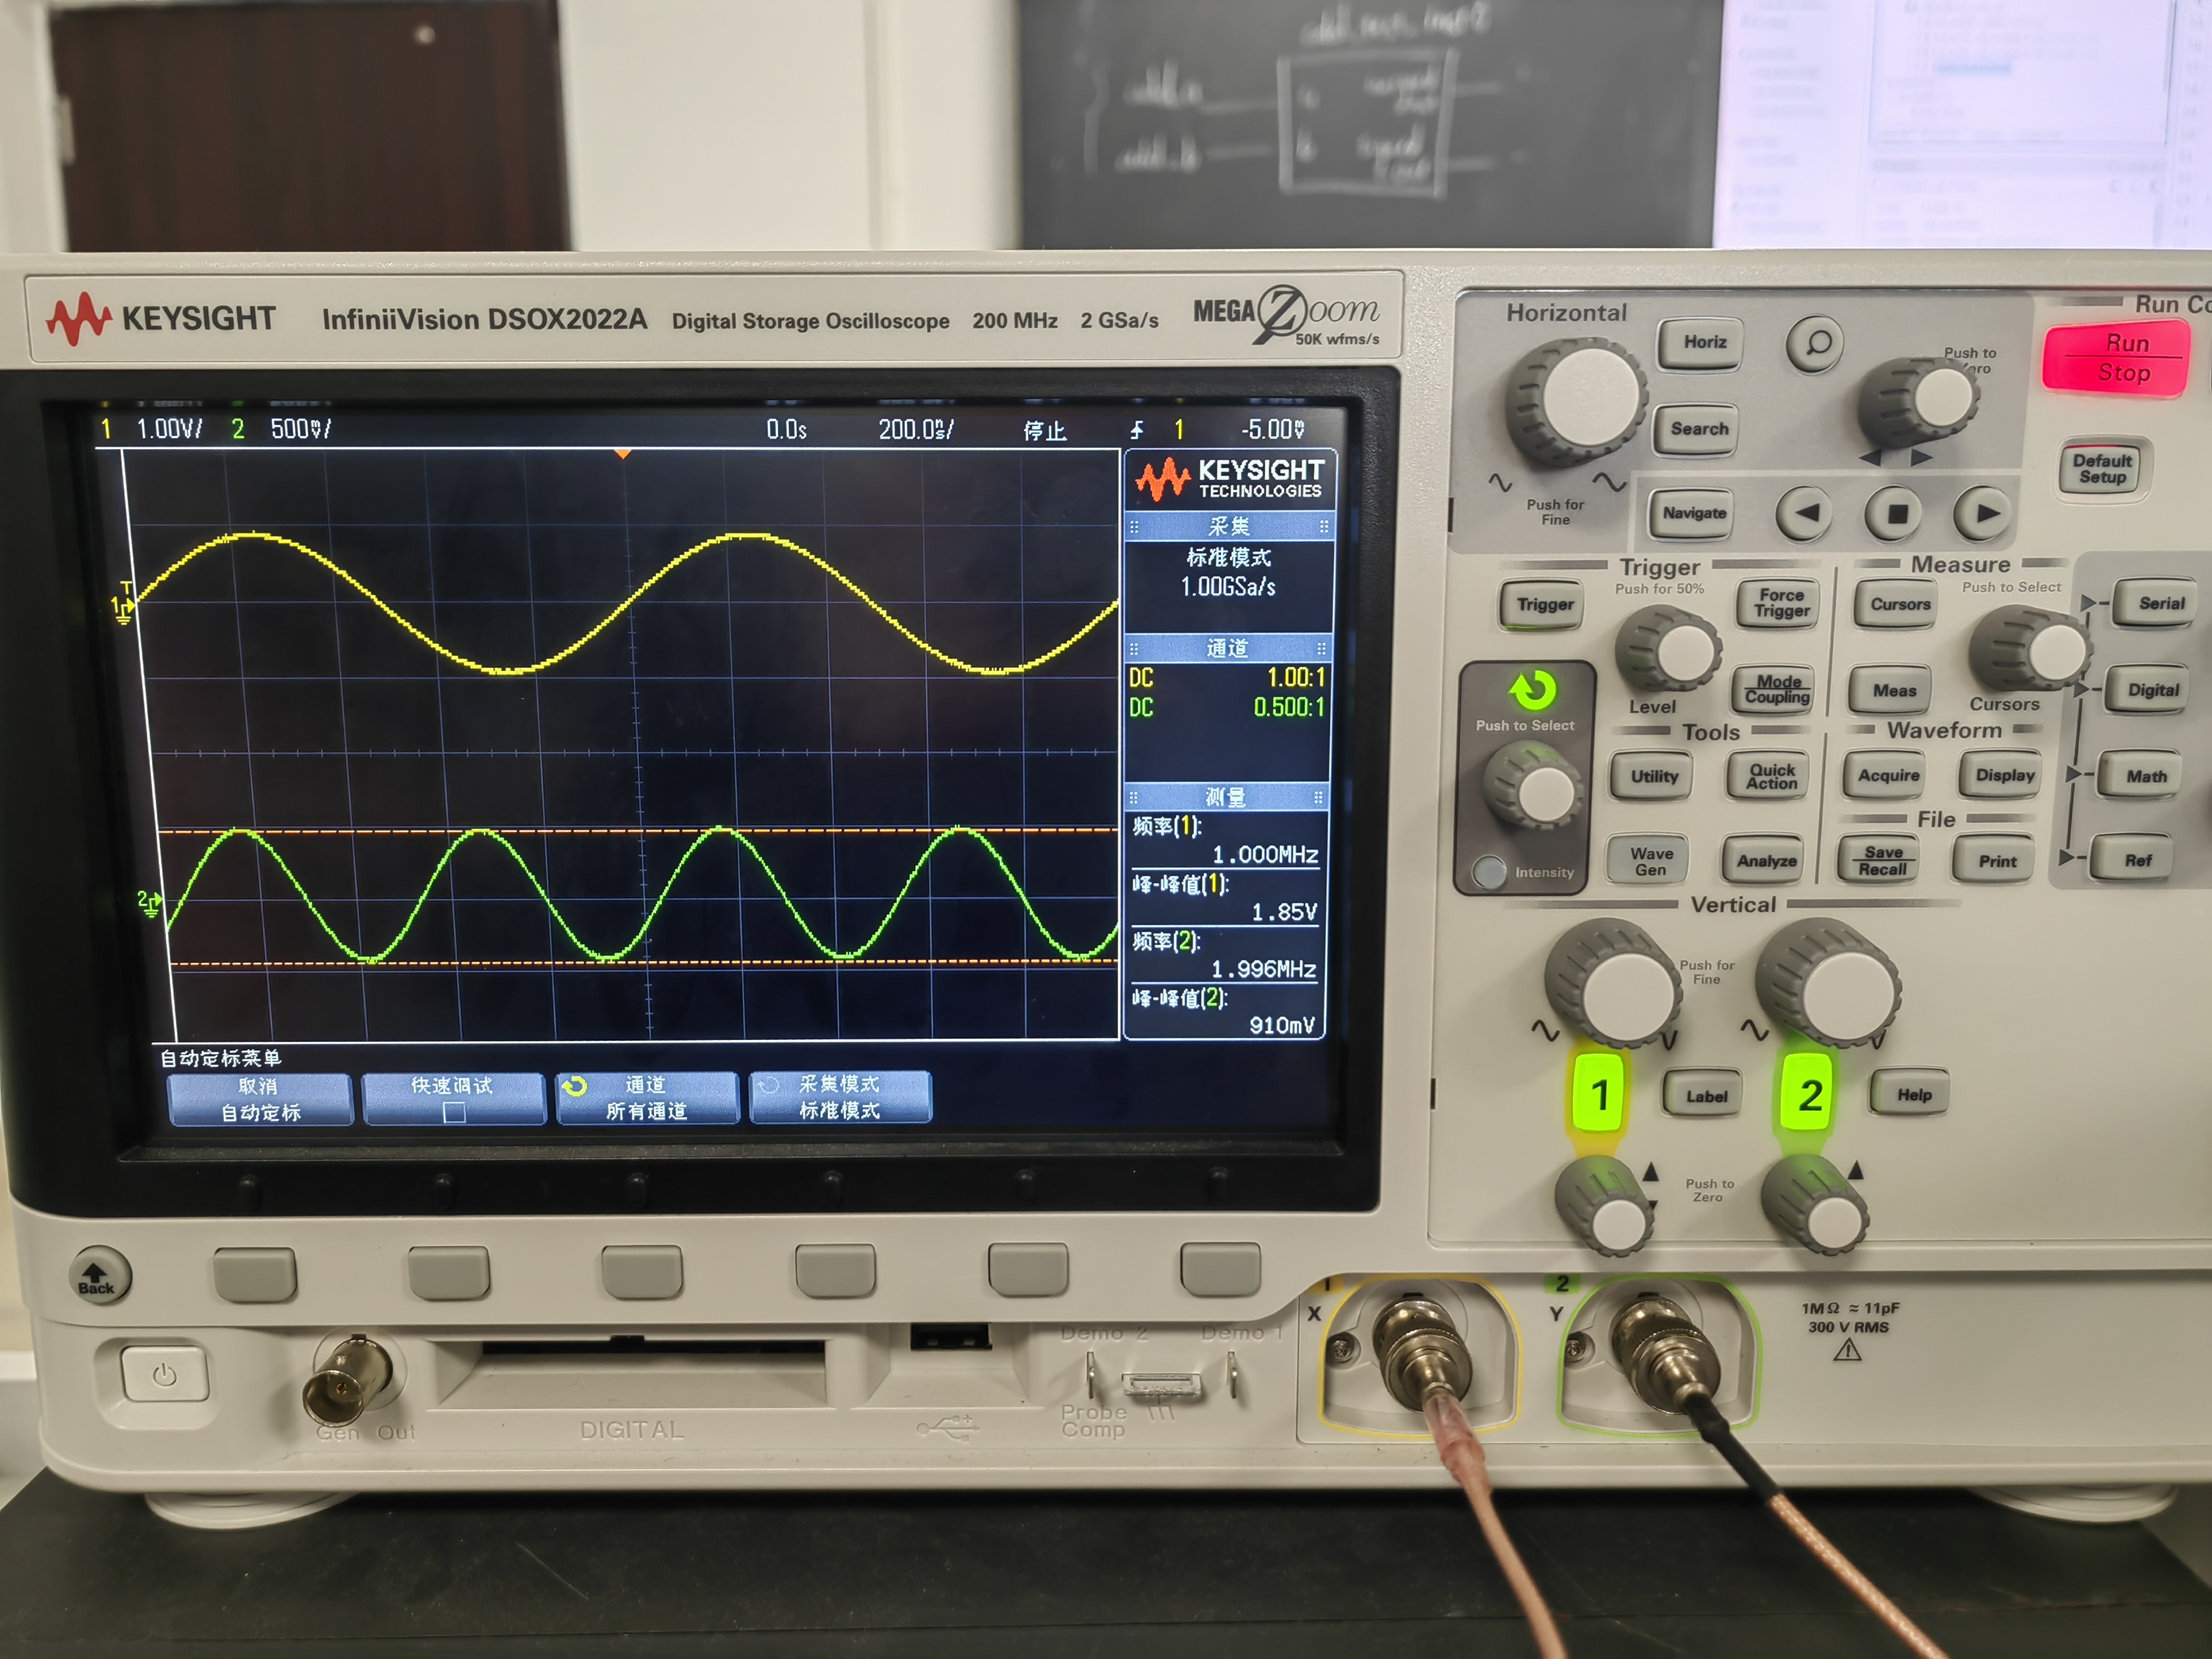
\includegraphics[width=0.75\textwidth]{figure/exp3/waveform.jpg}
  \caption{示波器波形}
  \label{fig:exp3:waveform}
\end{figure}

另外,在写入Bitstream之后,启动xsim,可以观察到ILA检测的两个余弦波的14-bit量化数据(即DAC之前的采样数据)如图~\ref{fig:exp3:sim}~。
\begin{figure}[htbp]
  \centering
  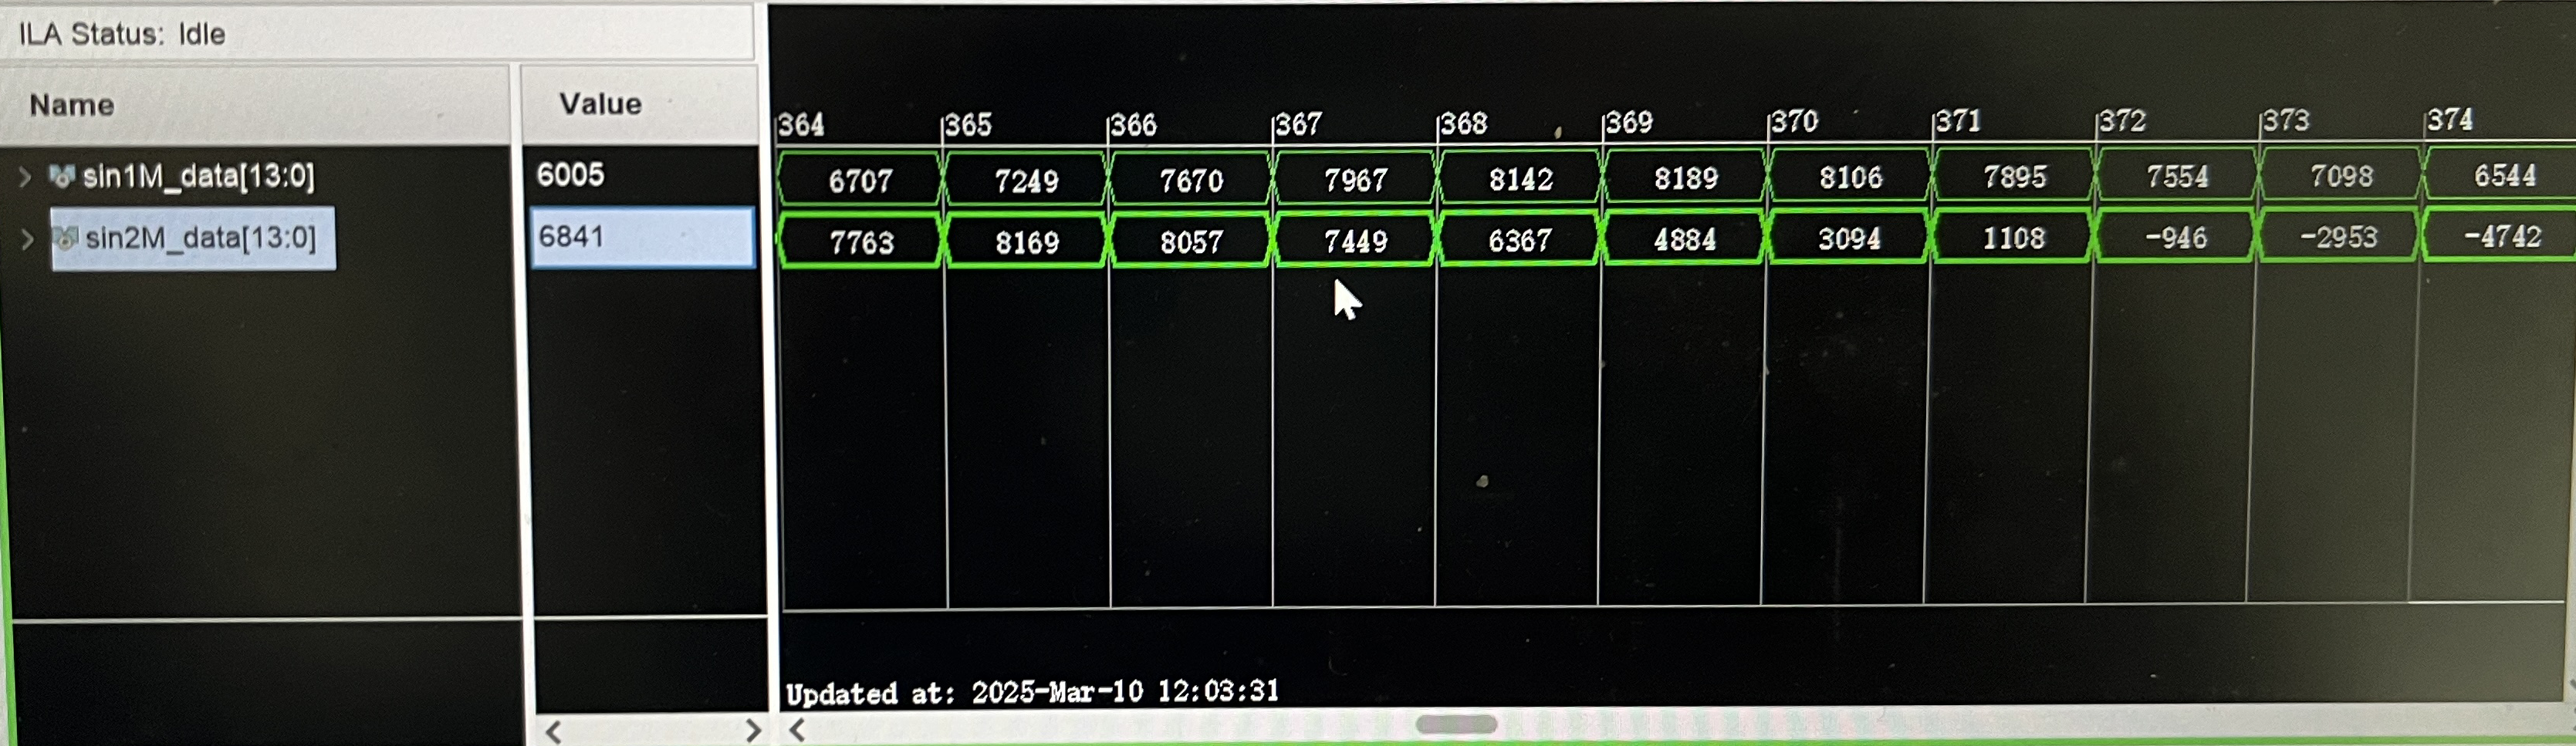
\includegraphics[width=0.75\textwidth]{figure/exp3/sim.png}
  \caption{余弦波的采样数据}
  \label{fig:exp3:sim}
\end{figure}
